\documentclass[12pt]{article}

% Packages
\usepackage[margin=1in]{geometry}
\usepackage{amsmath,amssymb,amsthm}
\usepackage{enumitem}
\usepackage{hyperref}
\usepackage{xcolor}
\usepackage{import}
\usepackage{xifthen}
\usepackage{pdfpages}
\usepackage{transparent}
\usepackage{listings}
\usepackage{tikz}
\usepackage{physics}
\usepackage{siunitx}
\usepackage{booktabs}
\usepackage{cancel}
\usetikzlibrary{positioning} % <- adds the “below=of …” key

  \usetikzlibrary{calc,patterns,arrows.meta,decorations.markings}


\DeclareMathOperator{\Log}{Log}
\DeclareMathOperator{\Arg}{Arg}
\DeclareMathOperator{\F}{F}
\DeclareMathOperator{\Aut}{Aut}


\lstset{
    breaklines=true,         % Enable line wrapping
    breakatwhitespace=false, % Wrap lines even if there's no whitespace
    basicstyle=\ttfamily,    % Use monospaced font
    frame=single,            % Add a frame around the code
    columns=fullflexible,    % Better handling of variable-width fonts
}

\newcommand{\incfig}[1]{%
    \def\svgwidth{\columnwidth}
    \import{./Figures/}{#1.pdf_tex}
}
\theoremstyle{definition} % This style uses normal (non-italicized) text
\newtheorem{solution}{Solution}
\newtheorem{proposition}{Proposition}
\newtheorem{problem}{Problem}
\newtheorem{lemma}{Lemma}
\newtheorem{theorem}{Theorem}
\newtheorem{remark}{Remark}
\newtheorem{note}{Note}
\newtheorem{definition}{Definition}
\newtheorem{example}{Example}
\newtheorem{corollary}{Corollary}
\theoremstyle{plain} % Restore the default style for other theorem environments
%

% Theorem-like environments
% Title information
\title{MATH 417 Practice Final Exam 1 Solutions}
\author{Jerich Lee}
\date{\today}

\begin{document}

\maketitle
\begin{solution}
  \textbf{Step--by--step solution.}  
  Throughout we work in $\Bbb Z_{4}=\{0,1,2,3\}$ with the binary operation  
  \[
     a\star b \;:=\; a+b+1 \pmod{4}.
  \]
  
  \begin{enumerate}
      \item[(a)] \emph{Cayley table.}  For each ordered pair $(a,b)$ compute
            $a+b+1$ modulo $4$:
  
            \[
            \renewcommand{\arraystretch}{1.2}
            \begin{array}{c|cccc}
                \star & 0 & 1 & 2 & 3\\\hline
                0 & 1 & 2 & 3 & 0\\
                1 & 2 & 3 & 0 & 1\\
                2 & 3 & 0 & 1 & 2\\
                3 & 0 & 1 & 2 & 3
            \end{array}
            \]
  
      \item[(b)] \emph{Identity element.}  
            An element $e$ is an identity iff $e\star a=a\star e=a$ for all
            $a\in G$.  
            From the last row \emph{and} last column of the table we see
            $3\star a=a\star 3=a$; hence the identity is
            \[
                 e=3.
            \]
  
      \item[(c)] \emph{Inverses.}  
            We need $a\star b=3=e$.  Solve $a+b+1\equiv 3\pmod 4$:
            \[
                b\equiv -a+2 \pmod 4.
            \]
            Hence
            \[
                0^{-1}=2,\qquad
                1^{-1}=1,\qquad
                2^{-1}=0,\qquad
                3^{-1}=3.
            \]
  
      \item[(d)] \emph{Check associativity for one non-trivial triple.}  
            Take $(a,b,c)=(1,2,0)$:
            \[
                (1\star 2)\star 0
                = 0 \star 0        % 1+2+1=4\equiv 0
                = 1,
                \qquad
                1\star(2\star 0)
                = 1\star 3          % 2+0+1=3
                = 1.
            \]
            The two results agree, illustrating associativity.
  
            (Indeed, \((a\star b)\star c = a+b+1+c+1
            \equiv a+b+c+2 \equiv a\star(b\star c)\), so the operation is
            associative for \emph{all} triples.)
  \end{enumerate}\qed
  \end{solution}
  \begin{solution}
    Let $G$ be a group and define the relation $\,\sim\,$ on $G$ by  
    \[
         a\;\sim\;b 
         \quad\Longleftrightarrow\quad 
         \exists\,g\in G \text{ such that } b = g a g^{-1}.
    \]
    The relation is called \emph{conjugacy}.  We address each part in turn.
    
    %--------------------------------------------------------------------
    \subsection*{(a)  $\sim$ is an equivalence relation}
    
    To show that $\sim$ is an equivalence relation, we must prove reflexivity, symmetry, and transitivity.
    
    \begin{itemize}
        \item\emph{Reflexive.}  
              For any $a\in G$, choose $g=e$ (the identity of $G$).  
              Then $gag^{-1}=e\,a\,e=a$, so $a\sim a$.
    
        \item\emph{Symmetric.}  
              Suppose $a\sim b$.  
              Then $b=gag^{-1}$ for some $g\in G$.  
              Multiply on the left by $g^{-1}$ and on the right by $g$:
              \[
                  a = g^{-1} b g,
              \]
              hence $b\sim a$ (with witness $g^{-1}$).
    
        \item\emph{Transitive.}  
              Suppose $a\sim b$ and $b\sim c$.  
              Then there exist $g_1,g_2\in G$ with
              \[
                  b=g_1 a g_1^{-1},
                  \qquad
                  c=g_2 b g_2^{-1}.
              \]
              Substituting the first equation into the second gives
              \[
                  c 
                  = g_2 \bigl(g_1 a g_1^{-1}\bigr) g_2^{-1}
                  = (g_2 g_1)\,a\,(g_2 g_1)^{-1},
              \]
              so $a\sim c$ (witness $g_2 g_1$).
    \end{itemize}
    Since $\sim$ is reflexive, symmetric, and transitive, it is an equivalence relation on~$G$.
    
    %--------------------------------------------------------------------
    \subsection*{(b)  Elements in the same conjugacy class have equal order}
    
    Assume $a,b\in G$ satisfy $a\sim b$; i.e.\ $b=gag^{-1}$ for some $g\in G$.
    Let $n:=\operatorname{ord}(a)$, so $a^{n}=e$ and $n$ is minimal with this property.
    Compute
    \[
          b^{\,n}
          = (gag^{-1})^{n}
          = g a^{n} g^{-1}
          = g e g^{-1}
          = e.
    \]
    Hence $\operatorname{ord}(b)$ divides $n$.  
    Repeating the argument with the roles of $a$ and $b$ reversed (using $g^{-1}$)
    shows that $\operatorname{ord}(a)$ divides $\operatorname{ord}(b)$.  
    Therefore $\operatorname{ord}(a)=\operatorname{ord}(b)$.
    
    \bigskip
    \noindent
    \textit{Conclusion:} conjugate elements not only lie in the same equivalence (conjugacy) class but also share the same order.
    \qed
    \end{solution}
    \begin{solution}
      \makeatletter\def\theenumi{\roman{enumi}}\def\labelenumi{(\theenumi)}\makeatother
      Let  
      \[
          C_{8}\;=\;\bigl\{\zeta_{8}^{\,k}\;:\;k=0,1,\dots,7\bigr\},
          \qquad
          \zeta_{8}:=e^{2\pi i/8}=e^{\pi i/4},
      \]
      with the usual complex multiplication.
      
      %--------------------------------------------------------------------
      \subsection*{(a)  $C_{8}$ is cyclic (hence abelian)}
      
      \begin{enumerate}
          \item $\boxed{\text{Order of }\zeta_{8}}$  
                Note $\zeta_{8}^{\,8}=e^{2\pi i}=1$.  
                If $\zeta_{8}^{\,m}=1$ for some $0<m<8$, then
                $e^{2\pi i m/8}=1\;\Longrightarrow\;8\mid m$, contradiction.
                Hence $\operatorname{ord}(\zeta_{8})=8$.
      
          \item $\boxed{\text{Generation}}$  
                Because $\zeta_{8}$ has order $8$, 
                \(
                    C_{8}=\langle\zeta_{8}\rangle.
                \)
      
          \item $\boxed{\text{Abelian}}$  
                A cyclic group is generated by a single element;
                for any $a=\zeta_{8}^{\,m}$ and $b=\zeta_{8}^{\,n}$
                we have $ab=\zeta_{8}^{\,m+n}=ba$.
      \end{enumerate}
      Thus $(C_{8},\cdot)$ is cyclic, and therefore abelian.
      
      %--------------------------------------------------------------------
      \subsection*{(b)  Subgroups and subgroup lattice}
      
      For a cyclic group of order $n$, there is a \emph{unique} subgroup of
      order $d$ for every divisor $d\mid n$.  
      The divisors of $8$ are $1,2,4,8$; hence
      
      \[
      \begin{array}{ccl}
      \text{order} & \text{subgroup} & \text{generator(s)}\\\hline
      1 & \{1\} & --\\
      2 & \langle\zeta_{8}^{4}\rangle=\{1,-1\} & \zeta_{8}^{4}\\
      4 & \langle\zeta_{8}^{2}\rangle=\{1,i,-1,-i\} & \zeta_{8}^{2},\;\zeta_{8}^{6}\\
      8 & C_{8} & \zeta_{8},\;\zeta_{8}^{3},\;\zeta_{8}^{5},\;\zeta_{8}^{7}
      \end{array}
      \]
      
      \smallskip
      \noindent
      \emph{Subgroup lattice:}
      
      \[
      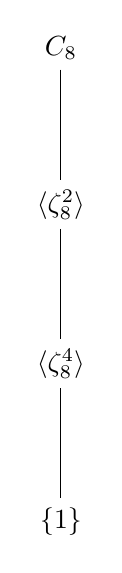
\begin{tikzpicture}[node distance=1.4cm]
         \node (C8)  {$C_{8}$};
         \node (H4)  [below=of C8] {$\langle\zeta_{8}^{2}\rangle$};
         \node (H2)  [below=of H4] {$\langle\zeta_{8}^{4}\rangle$};
         \node (H1)  [below=of H2] {$\{1\}$};
      
         \draw (C8) -- (H4) -- (H2) -- (H1);
      \end{tikzpicture}
      \]
      
      \noindent
      Each edge represents inclusion; no other subgroups exist.
      \qed
      \end{solution}
      \begin{solution}
        \begin{enumerate}[label=\textbf{(\alph*)}]
        
        %------------------------------------------------------------
        \item  \emph{Any subgroup of index $2$ is normal.}
        
        Let $G$ be a group and $H\le G$ with $[G:H]=2$.  
        Thus $H$ partitions $G$ into exactly two left cosets:
        \[
           G = H \sqcup gH
           \qquad(\text{for some } g\notin H).
        \]
        The right cosets form another partition
        \(
           G = H \sqcup Hg'.
        \)
        Because \emph{both} partitions consist of precisely the two subsets
        $H$ and $G\!\setminus\!H$, we must have
        \[
                gH = Hg'
                \quad\Longrightarrow\quad
                \forall x\in G:\;xH \in \{H,\,G\!\setminus\!H\}
                = \{H,\,Hx\}.
        \]
        Consequently the left and right cosets coincide for every $x\in G$,
        i.e.\ $xH = Hx$.  
        Therefore $H$ is normal:
        \[
           H \trianglelefteq G.
        \]
        
        \medskip
        
        %------------------------------------------------------------
        \item  \emph{A subgroup of index $3$ that is \textbf{not} normal.}
        
        Take $G=S_{3}$ (order $6$) and let
        \[
           H \;=\; \langle (12)\rangle
                \;=\; \bigl\{\,e,\,(12)\bigr\}.
        \]
        Then $|H|=2$, so $[G:H]=6/2 = 3$.
        
        To see that $H$ is \emph{not} normal, conjugate $(12)$ by $(13)$:
        \[
           (13)\,(12)\,(13)^{-1} \;=\; (13)(12)(13) = (23),
        \]
        but $(23)\notin H$.  
        Hence $(13)H(13)^{-1}\neq H$ and $H$ fails to be normal in~$S_{3}$.
        
        \end{enumerate}\qed
        \end{solution}
        \begin{solution}
          We write both groups additively:
          \[
             \mathbb{Z}_{15}=\bigl\langle 1\bigr\rangle,
             \qquad
             \mathbb{Z}_{6}=\{0,1,2,3,4,5\}.
          \]
          A group homomorphism $\varphi:\mathbb{Z}_{15}\to\mathbb{Z}_{6}$ must satisfy
          \[
             \varphi(m+n)=\varphi(m)+\varphi(n)\quad
             (m,n\in\mathbb{Z}_{15}).
          \]
          Because $\mathbb{Z}_{15}$ is \emph{cyclic}, \emph{every} homomorphism is completely
          determined by the image of the single generator~$1$:
          
          \[
                \boxed{\;
                \varphi(n)=n\cdot\varphi(1)\quad(n\in\mathbb{Z}_{15}).
                \;}
          \]
          
          %--------------------------------------------------------------------
          \subsection*{Step 1.  Compatibility condition}
          
          The relation $15\cdot 1=0$ in $\mathbb{Z}_{15}$ must be preserved, i.e. 
          \[
                \varphi(15\cdot 1)=15\cdot\varphi(1)=0\quad\text{in }\mathbb{Z}_{6}.
          \]
          Let $a:=\varphi(1)\in\mathbb{Z}_{6}$; then
          \[
                15a\equiv 0 \pmod{6}.
          \]
          Since $15\equiv 3\pmod 6$, the condition reduces to
          \[
                3a\equiv 0\pmod 6
                \;\Longleftrightarrow\;
                6\,\bigm|\,3a
                \;\Longleftrightarrow\;
                2\,\bigm|\,a.
          \]
          Thus $a$ must be \emph{even}.  The even elements of $\mathbb{Z}_{6}$ are
          \[
                a\in\{0,\,2,\,4\}.
          \]
          
          %--------------------------------------------------------------------
          \subsection*{Step 2.  Construct the homomorphisms}
          
          For each admissible $a$ define
          \[
               \varphi_{a} : \mathbb{Z}_{15}\longrightarrow \mathbb{Z}_{6},
               \qquad
               \varphi_{a}(n):=a\,n\pmod 6.
          \]
          Explicitly:
          \[
             \varphi_{0}(n)=0,   \qquad
             \varphi_{2}(n)=2n\pmod 6, \qquad
             \varphi_{4}(n)=4n\pmod 6.
          \]
          
          %--------------------------------------------------------------------
          \subsection*{Step 3.  Distinctness and counting}
          
          Two homomorphisms are equal iff their values on the generator~$1$ are
          equal.  Since $0,2,4$ are distinct in $\mathbb{Z}_{6}$, the three maps above are
          pairwise different.
          
          \[
             \boxed{\text{There are exactly $3$ group homomorphisms } \mathbb{Z}_{15}\to\mathbb{Z}_{6}.}
          \]
          
          \bigskip
          \noindent
          \textbf{Summary table}
          \[
          \renewcommand{\arraystretch}{1.2}
          \begin{array}{c|c|c|c}
          \text{image of $1$} & \varphi(1) & \varphi(5) & \varphi(15)\rule[-4pt]{0pt}{14pt}\\\hline
          0 & 0 & 0 & 0\\
          2 & 2 & 4 & 0\\
          4 & 4 & 2 & 0
          \end{array}
          \]
          
          \qed
          \end{solution}
        \begin{solution}
          Let $\Bbb Z_{15}=\langle 1\rangle$ and $\Bbb Z_{6}=\{0,1,2,3,4,5\}$ written additively.
          
          \medskip
          \textbf{Key observation.}  
          A homomorphism $\varphi:\mathbb{Z}_{15}\to\mathbb{Z}_{6}$ is completely determined by the image of the generator~$1$:
          \[
                  \varphi(n)=n\,\varphi(1)\quad\text{for every }n\in\mathbb{Z}_{15}.
          \]
          Conversely, any choice of $a:=\varphi(1)\in\mathbb{Z}_{6}$ that is \emph{compatible with the relation}
          $15\cdot 1 = 0$ in $\mathbb{Z}_{15}$ gives a homomorphism, provided
          \[
                  15a \equiv 0 \pmod{6}.
          \]
          
          \medskip
          \textbf{Solving $15a\equiv 0\;(\mathrm{mod}\;6)$.}\;
          Since $15\equiv 3\pmod 6$, the condition is
          \[
                  3a \equiv 0 \pmod 6
                  \quad\Longleftrightarrow\quad
                  6 \mid 3a
                  \quad\Longleftrightarrow\quad
                  2 \mid a.
          \]
          Thus $a$ must be a multiple of $2$ in $\mathbb{Z}_{6}$, i.e.\ 
          \[
             a\in\{0,\,2,\,4\}\subset\mathbb{Z}_{6}.
          \]
          
          \medskip
          \textbf{The homomorphisms.}\;
          For each admissible $a$ define
          \[
                \varphi_{a} :\mathbb{Z}_{15}\longrightarrow\mathbb{Z}_{6},
                \qquad
                \varphi_{a}(n):=a\,n \pmod 6.
          \]
          Explicitly:
          \[
          \varphi_{0}(n)=0,\qquad
          \varphi_{2}(n)=2n\pmod 6,\qquad
          \varphi_{4}(n)=4n\pmod 6.
          \]
          These are distinct because their values on $1$ differ.
          
          \medskip
          \textbf{Counting.}\;
          There are exactly \(\boxed{3}\) group homomorphisms
          \(\mathbb{Z}_{15}\to\mathbb{Z}_{6}\).
          \qed
          \end{solution}
          \begin{solution}
            Let $|G|=63=3^{2}\!\cdot 7$.
            
            %--------------------------------------------------------------------
            \subsection*{(a)  A unique (hence normal) Sylow $7$-subgroup}
            
            By Sylow’s theorems the number $n_{7}$ of Sylow $7$-subgroups satisfies  
            
            \[
                 n_{7}\;\bigm|\;9
                 \quad\text{and}\quad
                 n_{7}\equiv 1\pmod{7}.
            \]
            
            The divisors of $9$ are $\{1,3,9\}$; of these only $1$ is congruent to
            $1$ mod $7$.  Hence  
            \[
                    n_{7}=1.
            \]
            Thus $G$ contains a \emph{single} Sylow subgroup of order~$7$; call it $P$.
            Because it is the only conjugate of itself, $P$ is fixed by conjugation,
            hence normal:
            \[
                    P \trianglelefteq G .
            \]
            
            %--------------------------------------------------------------------
            \subsection*{(b)  $G$ need not be abelian}
            
            \paragraph{Strategy.}
            With $P\cong\Bbb Z_{7}$ normal, any Sylow $3$-subgroup $Q$ (order $9$)
            acts on $P$ by conjugation, giving a homomorphism
            \[
                    \phi : Q \longrightarrow \operatorname{Aut}(P)
                    \cong \Bbb Z_{6}.
            \]
            If $\phi$ is trivial the product is direct, $G\cong P\times Q$, and $G$
            is abelian; if $\phi$ is \emph{non-trivial}, the semidirect product
            $P\rtimes_{\phi} Q$ is \emph{non-abelian}.  We now show that such a
            non-trivial $\phi$ exists.
            
            \paragraph{Construction of a non-abelian group of order $63$.}
            Let $Q=\langle b\rangle\cong\Bbb Z_{9}$ and
            $P=\langle a\rangle\cong\Bbb Z_{7}$.
            Pick $k=2\in\Bbb Z_{7}^{\times}$; it has order $3$ because
            $2^{\,3}=8\equiv 1\pmod 7$.
            Define the action
            \[
                    b\,a\,b^{-1} \;=\; a^{k}=a^{2}.
            \]
            This extends uniquely to a homomorphism
            $\phi:Q\to\operatorname{Aut}(P)$ whose image has order~$3$ (non-trivial).
            Set
            \[
                    G \;=\; \langle\,a,b \mid
                            a^{7}=b^{9}=1,\;
                            b\,a\,b^{-1}=a^{2}\rangle
                    \;\cong\;
                    P\rtimes_{\phi} Q.
            \]
            
            Because $b$ does not commute with $a$ ($ba=a^{2}b$), $G$ is
            \emph{non-abelian}; nevertheless $|G|=7\cdot 9 = 63$.
            Hence:
            
            \[
               \boxed{\text{$G$ is \emph{not} necessarily abelian.}}
            \]
            
            \paragraph{Remark.}
            Every group of order $63$ is a semidirect product
            $P\rtimes Q$ as above; the action may be trivial (yielding the abelian
            group $\Bbb Z_{7}\times\Bbb Z_{9}$) or non-trivial (yielding the
            non-abelian example constructed here).  Thus both abelian and
            non-abelian groups of order $63$ exist.
            \qed
            \end{solution}
            %======================================================================
\subsection*{Expanded explanation for Part (b)}

Let $|G|=63=3^{2}\!\cdot 7$ and let $P\cong\mathbb{Z}_{7}$ be the \emph{unique}
(normal) Sylow $7$–subgroup found in part~(a).

\bigskip
%%%%%%%%%%%%%%%%%%%%%%%%%%%%%%%%%%%%%%%%%%%%%%%%%%%%%%%%%%%%%%%%%%%%%%%
\paragraph{\textbf{1.\;Using the Sylow $3$–subgroup to build $G$.}}

\begin{itemize}
\item Choose a Sylow $3$-subgroup $Q\le G$.
      By Sylow, $|Q|=9$ and $Q$ is \emph{not} normal in general.  
      Write $Q=\langle b\rangle\cong\mathbb{Z}_{9}$.

\item Conjugation by $Q$ induces a homomorphism  
      \[
            \phi : Q \;\longrightarrow\; \Aut(P).
      \]
      Because $P\cong\mathbb{Z}_{7}$ is cyclic, 
      \[
            \Aut(P)\;\cong\;\mathbb{Z}_{7}^{\times}\;\cong\;\mathbb{Z}_{6}
      \]
      (each unit $k\in\{1,\dots,6\}$ acts via $a\mapsto a^{k}$).
\end{itemize}

\medskip
%%%%%%%%%%%%%%%%%%%%%%%%%%%%%%%%%%%%%%%%%%%%%%%%%%%%%%%%%%%%%%%%%%%%%%%
\paragraph{\textbf{2.\;All possible $\phi$’s.}}

Since $\lvert Q\rvert=9$ and $\lvert\Aut(P)\rvert=6$,  
the image $\phi(Q)$ must divide $\gcd(9,6)=3$; 
so either $|\phi(Q)|=1$ (trivial action) or $|\phi(Q)|=3$ (non-trivial).

\begin{center}
\renewcommand{\arraystretch}{1.15}
\begin{tabular}{|c|c|l|}
\hline
$|\phi(Q)|$ & action & resulting group $P\rtimes_{\phi}Q$ \\\hline
$1$ & trivial & direct product $\,\mathbb{Z}_{7}\times\mathbb{Z}_{9}$ (abelian)\\
$3$ & non-trivial & semidirect product (non-abelian, see below)\\\hline
\end{tabular}
\end{center}

\medskip
%%%%%%%%%%%%%%%%%%%%%%%%%%%%%%%%%%%%%%%%%%%%%%%%%%%%%%%%%%%%%%%%%%%%%%%
\paragraph{\textbf{3.\;Constructing a non-trivial action.}}

Pick $k=2\in\mathbb{Z}_{7}^{\times}$;  
$2$ has order $3$ because $2^{3}=8\equiv1\pmod7$.  
Define
\[
        b\,a\,b^{-1}=a^{k}=a^{2},  
        \qquad  a\in P,\;b\in Q.
\]
This gives $\phi(b)=k$ and $\phi(Q)=\langle k\rangle$ of order $3$.

\smallskip
\emph{Presentation of the semidirect product:}
\[
   G_{\text{non-ab}}=
   \langle\,a,b \mid a^{7}=1,\;b^{9}=1,\;b\,a\,b^{-1}=a^{2}\rangle.
\]

Because $ba=a^{2}b\neq ab$, the group is \textbf{non-abelian}.  
Its order is $7\cdot9=63$ by the usual counting argument for semidirect
products.

\bigskip
%%%%%%%%%%%%%%%%%%%%%%%%%%%%%%%%%%%%%%%%%%%%%%%%%%%%%%%%%%%%%%%%%%%%%%%
\paragraph{\textbf{4.\;Why no other non-abelian possibilities arise.}}

\begin{itemize}
\item Any non-trivial action must map a generator of $Q$ to an element of
      $\Aut(P)\cong\mathbb{Z}_{6}$ of order $3$.
      There are two such elements, $k=2$ or $k=4$, but they are inverses
      in $\Aut(P)$, so the resulting semidirect products are isomorphic
      (relabel $b\mapsto b^{-1}$).

\item Therefore, \emph{up to isomorphism}, exactly \textbf{two} groups of
      order $63$ exist:

      \[
        \boxed{\mathbb{Z}_{7}\times\mathbb{Z}_{9}\quad\text{(abelian)}}
        \qquad\text{and}\qquad
        \boxed{\mathbb{Z}_{7}\rtimes_{\phi}\mathbb{Z}_{9}\quad\text{(non-abelian)}}.
      \]
\end{itemize}

\bigskip
%%%%%%%%%%%%%%%%%%%%%%%%%%%%%%%%%%%%%%%%%%%%%%%%%%%%%%%%%%%%%%%%%%%%%%%
\paragraph{\textbf{5.\;Take-away.}}

* A normal Sylow subgroup does \emph{not} force the whole group to be abelian;  
  it merely allows the group to be expressed as a semidirect product.

* The action of $Q$ on $P$ is encoded by a homomorphism
  $Q\to\Aut(P)$; the kernel of this map distinguishes the abelian and
  non-abelian cases.

\[
\boxed{\text{Hence groups of order }63\text{ can be abelian or non-abelian.}}
\]

\noindent
(For exam purposes, remember the recipe:  
choose $a^{7}=1$, $b^{9}=1$, set $ba=a^{2}b$, and you have a quick example
of a non-abelian group of order $63$.)
\paragraph{Why must \(\lvert\phi(Q)\rvert\mid 3\)?}
The map
\[
     \phi : Q \;\longrightarrow\; \Aut(P)
\]
is a group homomorphism with  

\[
     |Q| = 9,
     \qquad
     |\Aut(P)| = 6.
\]

\begin{enumerate}[label=\textit{\arabic*.},wide,labelwidth=0pt,labelsep=.8em]
    \item \textbf{Image divides the domain’s order.}\;
          By the First Isomorphism Theorem,
          \(
                Q/\ker\phi \;\cong\; \phi(Q)
          \).
          Hence
          \(
                \lvert\phi(Q)\rvert \mid |Q| = 9.
          \)

    \item \textbf{Image divides the codomain’s order.}\;
          Because \(\phi(Q)\le\Aut(P)\),
          Lagrange’s theorem gives
          \(
                \lvert\phi(Q)\rvert \mid |\Aut(P)| = 6.
          \)
\end{enumerate}

Combining the two divisibility conditions,
\[
       \lvert\phi(Q)\rvert \;\bigm|\; \gcd(9,6)=3.
\]
Since \(3\) is prime, the only possibilities are
\[
       \boxed{\lvert\phi(Q)\rvert=1 \quad\text{or}\quad \lvert\phi(Q)\rvert=3.}
\]

\smallskip
* If \(\lvert\phi(Q)\rvert=1\) (trivial action) one gets the direct product
  \(\mathbb{Z}_{7}\times\mathbb{Z}_{9}\) (abelian).  
* If \(\lvert\phi(Q)\rvert=3\) (non-trivial action) one obtains a
  non-abelian semidirect product of order \(63\).
  \paragraph{Why we chose the rule $\,b\,a\,b^{-1}=a^{2}\,$ (and why it is \emph{not} arbitrary).}

\medskip
\textbf{1.  What must a non-trivial action look like?}

\[
   \phi \;:\; Q=\langle b\rangle\cong\mathbb{Z}_{9} \;\longrightarrow\;
   \Aut(P)\cong\mathbb{Z}_{6},
\qquad P=\langle a\rangle\cong\mathbb{Z}_{7}.
\]

* We want $\phi$ to have image of order \(3\).  
  That forces \(\ker\phi\) to have order \(9/3=3\) (First Iso.\ Thm.).  
  In particular, \(b^{3}\in\ker\phi\).

* Inside \(\Aut(P)\cong\mathbb{Z}_{6}=\{1,2,3,4,5\}\) (written additively),
  the elements of order \(3\) are precisely \(2\) and \(4\)
  (since \(2\cdot3\equiv0\equiv4\cdot3\pmod 6\)).

* Therefore \emph{any} non-trivial action amounts to choosing one of
  those order-\(3\) automorphisms and declaring
  \[
       \phi(b)=2 
       \quad\text{or}\quad
       \phi(b)=4
       \qquad
       (\text{mod }6).
  \]

\medskip
\textbf{2.  Translating $\phi$ into a conjugation rule.}

* Recall: $\Aut(P)$ acts by $k:a\mapsto a^{k}$.
* Taking $k=2$ means “\(\phi(b)\) sends $a$ to $a^{2}$”,
  i.e.\ \(b\,a\,b^{-1}=a^{2}\).

\medskip
\textbf{3.  Why $k=2$ is as good as $k=4$.}

* If we had chosen \(k=4\) we would get the rule
  \(b\,a\,b^{-1}=a^{4}\).  
* But \(4\equiv2^{-1}\pmod 7\); relabeling \(b\mapsto b^{-1}\)
  swaps the two choices, and the resulting semidirect products are
  isomorphic.  
  Hence picking $k=2$ is simply the \emph{simplest} representative.

\medskip
\textbf{4.  Summary.}

The conjugation law \(b\,a\,b^{-1}=a^{2}\)

* realises an automorphism of order \(3\) on \(P\),
* gives the image \(|\phi(Q)|=3\),
* guarantees the product \(\,P\rtimes_{\phi}Q\) is non-abelian.

It is \textbf{forced by the group-theoretic constraints}—
not random decoration.
\paragraph{Why $\displaystyle \Aut(P)\;\cong\;\Bbb Z_{7}^{\times}\;\cong\;\Bbb Z_{6}$}

Let $P=\langle a\rangle$ be a cyclic group of order $7$
(\,$P\cong\Bbb Z_{7}$\,).  We describe \(\Aut(P)\) explicitly.

\smallskip
\textbf{1.\;Automorphisms are determined by the image of the generator.}

An automorphism \(\sigma\in\Aut(P)\) must send the generator \(a\) to
another generator of \(P\); otherwise \(\sigma\) would not be surjective.
Every generator of \(P\) has the form \(a^{k}\) with
\(1\le k\le 6\) and \(\gcd(k,7)=1\).

\smallskip
\textbf{2.\;Action described by an exponent $k$.}

Conversely, for any integer \(k\) with \(\gcd(k,7)=1\)
define
\[
      \sigma_{k}(a^{m}) \;:=\; a^{km}\quad(m\in\Bbb Z).
\]
Because \(k\) is invertible modulo \(7\),
\(\sigma_{k}\) is bijective and hence lies in \(\Aut(P)\).

\smallskip
\textbf{3.\;Establish the isomorphism.}

The assignment
\[
      k\pmod{7}
      \;\longmapsto\; \sigma_{k}
\]
is a homomorphism
\(
      \Bbb Z_{7}^{\times}\to\Aut(P)
\)
and it is bijective by construction.
Thus
\[
      \boxed{\Aut(P)\;\cong\;\Bbb Z_{7}^{\times}}.
\]

\smallskip
\textbf{4.\;$\Bbb Z_{7}^{\times}$ is cyclic of order $6$.}

For any prime \(p\), the multiplicative group
\(
      \Bbb Z_{p}^{\times}
\)
is cyclic of order \(p-1\).
Hence \(\Bbb Z_{7}^{\times}\cong\Bbb Z_{6}\).

\[
      \boxed{\Aut(P)\;\cong\;\Bbb Z_{6}}
\]

\noindent
(In fact \(3\) or \(5\) is a generator of \(\Bbb Z_{7}^{\times}\); the
corresponding automorphism \(a\mapsto a^{3}\) has order~\(6\).)
\begin{theorem}[Primitive‐root theorem]
  For every prime\/ $p$ the multiplicative group
  \[
        \Bbb Z_{p}^{\times}
        \;=\;
        \{\,1,2,\dots ,p-1\}
  \]
  is \emph{cyclic}.  Consequently it has order $p-1$ and possesses
  $\varphi(p-1)$ generators (the \emph{primitive roots modulo $p$}).
  \end{theorem}
  
  \begin{proof}
  Because $\Bbb Z_{p}$ is a field, $\Bbb Z_{p}^{\times}$ is a finite
  abelian group of order $p-1$.
  By the Fundamental Theorem of Finite Abelian Groups it is a direct
  product of cyclic $p$–power–free components,
  \[
        \Bbb Z_{p}^{\times}\;\cong\;
        C_{d_{1}}\;\oplus\;C_{d_{2}}\;\oplus\;\dots\;\oplus\;C_{d_{r}}
        \quad(d_{1}\mid d_{2}\mid\cdots\mid d_{r}).
  \]
  We will show $r=1$, i.e.\ the group is already cyclic.
  
  \medskip
  \textit{Step 1 – Each prime divisor occurs once.}
  Fix a prime $q\mid(p-1)$ and let
  \[
         A_q \;=\; \{\,x\in\Bbb Z_{p}^{\times} : x^{(p-1)/q}=1\,\}.
  \]
  $A_q$ is a subgroup, hence $|A_q|$ divides $p-1$.
  But its defining equation has degree $(p-1)/q$ and lives in a field of
  characteristic $p$, so by the factor theorem it has at most
  $(p-1)/q$ roots.  Thus $|A_q|\le(p-1)/q$.
  On the other hand the map $x\mapsto x^{(p-1)/q}$ is a homomorphism
  $\Bbb Z_{p}^{\times}\to\Bbb Z_{p}^{\times}$ whose image is $A_q$, so by
  Lagrange $|A_q|=(p-1)/q$ exactly.  Hence every prime divisor $q$ of
  $p-1$ appears with multiplicity \emph{one} in the invariant factor
  decomposition.
  
  \smallskip
  \textit{Step 2 – Direct product of pairwise coprime cyclic groups is cyclic.}
  Write $p-1=q_{1}q_{2}\cdots q_{k}$ (distinct primes).
  From Step 1,
  \[
       \Bbb Z_{p}^{\times}\;\cong\;
       C_{q_{1}}\;\oplus\;C_{q_{2}}\;\oplus\;\dots\;\oplus\;C_{q_{k}}.
  \]
  Because the moduli $q_{i}$ are pairwise coprime, the direct product is
  itself cyclic (Chinese remainder argument), generated for instance by an
  element whose components generate each $C_{q_{i}}$.
  
  \smallskip
  \textit{Conclusion.}
  Therefore $\Bbb Z_{p}^{\times}$ is cyclic of order $p-1$.
  \end{proof}
%======================================================================
            \begin{solution}
              We use the Fundamental Theorem of Finite Abelian Groups, which states  
              that every finite abelian group factors uniquely (up to isomorphism and
              ordering of the factors) into a direct product of primary cyclic groups.
              
              \medskip
              \textbf{Factor the order.}\;
              \[
                    84 \;=\; 2^{2}\;\cdot\;3\;\cdot\;7 .
              \]
              
              \begin{enumerate}[label=\textbf{\arabic*.},wide,labelwidth=0pt,labelsep=1em]
              
              %--------------------------------------------------------------------
              \item \textbf{$2$–primary part.}\;
                    Order $2^{2}=4$.
                    The partitions of the exponent $2$ give the options  
                    \[
                         \mathbb{Z}_{4},
                         \qquad
                         \mathbb{Z}_{2}\oplus\mathbb{Z}_{2}.
                    \]
              
              %--------------------------------------------------------------------
              \item \textbf{$3$–primary part.}\;
                    Order $3$.
                    Only \(\mathbb{Z}_{3}\).
              
              %--------------------------------------------------------------------
              \item \textbf{$7$–primary part.}\;
                    Order $7$.
                    Only \(\mathbb{Z}_{7}\).
              \end{enumerate}
              
              \medskip
              \textbf{Assemble the products.}\;
              Because $4,3,7$ are pairwise coprime,
              the direct product of the primary parts is already the full group.
              
              \[
              \boxed{\;
              \begin{aligned}
                 G_{1} &\;\cong\;
                         \mathbb{Z}_{4}\;\oplus\;\mathbb{Z}_{3}\;\oplus\;\mathbb{Z}_{7}
                         &&\cong\;\mathbb{Z}_{84},
                 \\[4pt]
                 G_{2} &\;\cong\;
                         \mathbb{Z}_{2}\;\oplus\;\mathbb{Z}_{2}\;\oplus\;\mathbb{Z}_{3}\;\oplus\;\mathbb{Z}_{7}
                         &&\cong\;\mathbb{Z}_{2}\;\oplus\;\mathbb{Z}_{2}\;\oplus\;\mathbb{Z}_{21}.
              \end{aligned}
              \;}
              \]
              
              \smallskip
              No other combinations are possible, so there are exactly
              \(\boxed{2}\) pairwise non-isomorphic abelian groups of order $84$.
              \qed
              \end{solution}
              \begin{solution}
                Write $\mathbb{Z}_{20}^{\ast}$ for the multiplicative group of units modulo $20$.
                
                \[
                   \mathbb{Z}_{20}^{\ast}
                   \;=\;
                   \{\,a\in\{1,\dots,19\}\mid\gcd(a,20)=1\}
                   \;=\;
                   \{1,3,7,9,11,13,17,19\}.
                \]
                
                Because $|\mathbb{Z}_{20}^{\ast}|=\varphi(20)=8$, every element has order dividing $8$.
                
                %------------------------------------------------------------------
                \subsection*{(a)  Order of each element}
                
                \vspace{-6pt}
                \renewcommand{\arraystretch}{1.15}
                \begin{center}
                \begin{tabular}{c|c|c}
                $a$ & first non–trivial power equal to $1$ & ${\rm ord}_{\mathbb{Z}_{20}^{\ast}}(a)$\\\hline
                $1$  & $1^{1}\equiv 1$                                     & $1$\\
                $3$  & $3^{4}=81\equiv 1\pmod{20}$ ($3^{2}=9\neq 1$)       & $4$\\
                $7$  & $7^{4}=81\equiv 1\pmod{20}$ ($7^{2}=9\neq 1$)       & $4$\\
                $9$  & $9^{2}=81\equiv 1\pmod{20}$                         & $2$\\
                $11$ & $11^{2}=121\equiv 1\pmod{20}$                       & $2$\\
                $13$ & $13^{4}=81\equiv 1\pmod{20}$ ($13^{2}=9\neq 1$)     & $4$\\
                $17$ & $17^{4}=81\equiv 1\pmod{20}$ ($17^{2}=9\neq 1$)     & $4$\\
                $19$ & $19^{2}=361\equiv 1\pmod{20}$                       & $2$
                \end{tabular}
                \end{center}
                
                \[
                \boxed{
                \begin{aligned}
                &\operatorname{ord}(1)=1;\\
                &\operatorname{ord}(3)=\operatorname{ord}(7)=\operatorname{ord}(13)=\operatorname{ord}(17)=4;\\
                &\operatorname{ord}(9)=\operatorname{ord}(11)=\operatorname{ord}(19)=2.
                \end{aligned}}
                \]
                
                %------------------------------------------------------------------
                \subsection*{(b)  Generators of $\mathbb{Z}_{20}^{\ast}$}
                
                A \emph{generator} is an element whose order equals the order of the
                group.  
                Since the largest order we found is $4<8=|\mathbb{Z}_{20}^{\ast}|$,  
                \[
                   \text{no element of }\mathbb{Z}_{20}^{\ast}\text{ has order }8.
                \]
                Hence $\mathbb{Z}_{20}^{\ast}$ is \emph{not cyclic} and admits
                \[
                   \boxed{\text{no (single) generators.}}
                \]
                
                (Indeed $\mathbb{Z}_{20}^{\ast}\cong\mathbb{Z}_{4}\times\mathbb{Z}_{2}$, a direct product of
                smaller cyclic groups.)
                \qed
                \end{solution}
                \begin{solution}
                  \textbf{(a)  Wilson’s Theorem.}  
                  Let $p$ be an \emph{odd} prime.  
                  Work in the multiplicative group $\mathbb{Z}_{p}^{\times}=\{1,2,\dots ,p-1\}$,
                  which is of order $p-1$.
                  
                  \smallskip
                  \textit{Step 1 – Pair every element with its inverse.}  
                  For each $a\in\mathbb{Z}_{p}^{\times}$ there exists a \emph{unique} inverse
                  $a^{-1}\in\mathbb{Z}_{p}^{\times}$ such that $aa^{-1}\equiv 1\pmod{p}$.
                  Moreover
                  \[
                         a\equiv a^{-1}\pmod{p}
                         \;\Longrightarrow\;
                         a^{2}\equiv 1
                         \;\Longrightarrow\;
                         p\,\bigm|\,a^{2}-1=(a-1)(a+1),
                  \]
                  so $a\equiv \pm1\pmod{p}$.  
                  Hence the \emph{only} elements that are their own inverses are
                  $1$ and $p-1$.
                  
                  \smallskip
                  \textit{Step 2 – Multiply all elements.}  
                  Take the product of all residues:
                  \[
                        (p-1)!
                        \;=\;
                        1\cdot 2\cdots(p-2)\cdot(p-1)
                        \;\equiv\;
                        \bigl(1\bigr)\bigl(p-1\bigr)
                          \!\!\!\!
                          \prod_{\substack{2\le a\le p-2\\ a^{-1}\neq a}}
                          \!\!\!\! (aa^{-1})
                        \pmod{p}.
                  \]
                  Each term $aa^{-1}$ in the product over pairs contributes $1$.
                  Thus
                  \[
                        (p-1)!\;\equiv\; 1\cdot(p-1)\;\equiv\;-1\pmod{p}.
                  \]
                  
                  \smallskip
                  \textit{Conclusion.}\;
                  For every odd prime $p$,
                  \[
                        \boxed{(p-1)! \equiv -1 \pmod{p}}.
                  \]
                  
                  %--------------------------------------------------------------------
                  \bigskip
                  \textbf{(b)  Evaluate $12!\pmod{13}$.}
                  
                  Set $p=13$ (an odd prime).  
                  By part (a),
                  \[
                        12! = (13-1)! \equiv -1 \pmod{13}.
                  \]
                  Since $-1\equiv 12\pmod{13}$,
                  \[
                        \boxed{12!\equiv 12 \pmod{13}}.
                  \]
                  \qed
                  \end{solution}
                  \begin{solution}
                    %==============================================================
                    \textbf{(a)  Every finite integral domain is a field}
                    
                    Let $R$ be a finite integral domain (commutative ring with $1\neq 0$ and
                    no zero–divisors).
                    
                    \smallskip
                    \emph{Goal.}  Show that every non–zero $a\in R$ is \underline{invertible}.
                    
                    \begin{enumerate}[label=\textit{Step \arabic*:},wide,labelwidth=0pt,labelsep=.8em]
                        \item \textbf{Injective multiplication map.}
                              Fix $a\neq 0$ and consider  
                              \[
                                  \mu_{a} : R \longrightarrow R, 
                                  \qquad
                                  \mu_{a}(x):=ax .
                              \]
                              If $\mu_{a}(x)=\mu_{a}(y)$ then $ax=ay$ and
                              $a(x-y)=0$.  
                              Because $R$ has no zero–divisors and $a\neq 0$, we must
                              have $x-y=0$, so $x=y$.  
                              Thus $\mu_{a}$ is \emph{injective}.
                    
                        \item \textbf{Injective $\;\Rightarrow\;$ surjective (finite set!).}
                              The set $R$ is finite, so an injective self–map is automatically
                              surjective.  
                              Hence there exists $b\in R$ with $\mu_{a}(b)=1$, i.e.\ $ab=1$.
                    
                        \item \textbf{Invertibility.}
                              The element $b$ is a (two–sided) multiplicative inverse of $a$.
                              Since $a\neq 0$ was arbitrary, \emph{every} non–zero element of
                              $R$ is invertible.
                    \end{enumerate}
                    
                    Therefore $R$ satisfies the definition of a field:
                    \[
                       \boxed{\text{finite integral domain } \Longrightarrow \text{ field}.}
                    \]
                    
                    %==============================================================
                    \bigskip
                    \textbf{(b)  A finite ring that is \emph{not} an integral domain}
                    
                    Take the ring $\displaystyle R=\Bbb Z_{6}=\{0,1,2,3,4,5\}$ with ordinary
                    addition and multiplication modulo $6$.
                    
                    \begin{itemize}
                        \item $R$ is finite and has identity $1$.
                    
                        \item Zero–divisors:
                              \[
                                 2\cdot 3 \equiv 0,\quad
                                 2\cdot 0 \equiv 0,\quad
                                 3\cdot 4 \equiv 0,\quad
                                 4\cdot 3 \equiv 0.
                              \]
                              Hence the non–zero zero–divisors are
                              \[
                                   \boxed{\;2,\;3,\;4\;}
                              \]
                              (together with $0$ itself).
                              The presence of zero–divisors means $\mathbb{Z}_{6}$ is \emph{not} an
                              integral domain.
                    \end{itemize}
                    
                    Thus $\mathbb{Z}_{6}$ is a concrete finite ring with identity that fails to be
                    an integral domain, and its full set of zero–divisors is
                    $\{0,2,3,4\}$.
                    \qed
                    \end{solution}
                    \begin{solution}
                      Let $\Bbb Z[i]=\{a+bi\mid a,b\in\Bbb Z\}$ be the ring of Gaussian integers
                      and let 
                      \[
                           N(a+bi):=(a+bi)(a-bi)=a^{2}+b^{2}\quad(a,b\in\Bbb Z)
                      \]
                      be the \emph{norm}.
                      
                      %------------------------------------------------------------
                      \subsection*{(a)  $\Bbb Z[i]$ is a Euclidean domain}
                      
                      A Euclidean domain is an integral domain in which there is a map
                      $\delta:R\setminus\{0\}\to\Bbb N$ such that for all
                      $\alpha,\beta\in R$ with $\beta\ne 0$ there exist
                      $q,r\in R$ satisfying 
                      \[
                              \alpha=\beta q+r,
                              \qquad
                              r=0\text{ or }\delta(r)<\delta(\beta).
                      \]
                      
                      \begin{enumerate}[label=\textit{Step \arabic*:},wide, labelwidth=0pt,labelsep=.8em]
                          \item\textbf{Integral domain.}\;
                                $\Bbb Z[i]$ is a subring of $\Bbb C$ with no zero–divisors.
                      
                          \item\textbf{Division with remainder.}\;
                                Given $\alpha,\beta\in\Bbb Z[i]$ ($\beta\ne 0$) write
                                $\alpha/\beta = x+yi\in\Bbb C$.
                                Choose integers $m,n$ with 
                                $\bigl|x-m\bigr|\le\frac12$ and $\bigl|y-n\bigr|\le\frac12$
                                (round the real and imaginary parts).
                                Let $q:=m+ni\in\Bbb Z[i]$ and set
                                \[
                                      r:=\alpha-\beta q.
                                \]
                                Then 
                                \(
                                      r = \beta(x+yi-q) = \beta\varepsilon
                                \)
                                where $\varepsilon=(x-m)+(y-n)i$ satisfies
                                $|\varepsilon|\le\frac{\sqrt{2}}{2}<1$.  Hence
                                \[
                                       N(r)=N(\beta)\,|\varepsilon|^{2}
                                               < N(\beta).
                                \]
                                This gives the required division algorithm with $\delta=N$.
                      
                      \end{enumerate}
                      Therefore $(\Bbb Z[i],+,\cdot)$ is a Euclidean domain (hence a PID and UFD).
                      
                      %------------------------------------------------------------
                      \subsection*{(b)  $\gcd(4+5i,\;7+2i)$ in $\Bbb Z[i]$}
                      
                      Apply the Euclidean algorithm.
                      
                      \medskip\noindent
                      \textit{First step.}
                      \[
                         \frac{7+2i}{4+5i}
                         =\frac{(7+2i)(4-5i)}{41}
                         =\frac{38-27i}{41}
                         \approx 0.93-0.66i.
                      \]
                      Nearest Gaussian integer: $q_{1}=1-i$.
                      \[
                         r_{1}=(7+2i)-(1-i)(4+5i)=(7+2i)-(9+i)=-2+i,\qquad N(r_{1})=5.
                      \]
                      
                      \medskip\noindent
                      \textit{Second step.}
                      \[
                         \frac{4+5i}{-2+i}
                         =\frac{(4+5i)(-2-i)}{5}
                         =\frac{-3-14i}{5}
                         \approx-0.6-2.8i.
                      \]
                      Nearest Gaussian integer: $q_{2}=-1-3i$.
                      \[
                         r_{2}=(4+5i)-(-1-3i)(-2+i)=(4+5i)-(5+5i)=-1,\qquad N(r_{2})=1.
                      \]
                      
                      \medskip\noindent
                      \textit{Third step.}\;
                      $(-2+i)=(-1) \cdot (-1) + 0$.
                      
                      The last non–zero remainder is $-1$, whose norm $1$ is minimal.
                      Up to multiplication by the unit group $\{\pm1,\pm i\}$ the gcd is~$1$.
                      
                      \[
                            \boxed{\gcd_{\Bbb Z[i]}(4+5i,\;7+2i)=1}.
                      \]
                      
                      \noindent(The two numbers are \emph{coprime} in $\Bbb Z[i]$.)
                      \qed
                      \end{solution}
                      \begin{solution}
                        Let $p$ be prime and let 
                        \[
                                V \;=\; \mathbb{Z}_{p}\;\oplus\;\mathbb{Z}_{p}
                        \]
                        written additively.  View $\mathbb{Z}_{p}$ as the finite field
                        $\F_{p}$.  Then $V$ is a $2$-dimensional vector space over~$\F_{p}$.
                        
                        %--------------------------------------------------------------------
                        \subsection*{(a)  $\operatorname{Aut}(V)\;\cong\;GL_{2}(\F_{p})$}
                        
                        \paragraph{(i)  Each automorphism is $\F_{p}$-linear.}
                        Take $\varphi\in\operatorname{Aut}(V)$.
                        Because $V$ is an \emph{elementary} abelian $p$-group, every element has order
                        $p$ and hence
                        \[
                                p\cdot v = 0\quad\text{for all }v\in V.
                        \]
                        Applying $\varphi$ gives $p\cdot\varphi(v)=0$, so $\varphi(v)$ also has
                        order dividing $p$, i.e.\ lies in $V$.  
                        Moreover, for any $a\in\F_{p}$ and $v,w\in V$,
                        \[
                                \varphi(v+w)=\varphi(v)+\varphi(w),
                                \qquad
                                \varphi(a\cdot v)
                                = \underbrace{v+\dots+v}_{a\text{ times}}
                                  \mapsto
                                  \underbrace{\varphi(v)+\dots+\varphi(v)}_{a\text{ times}}
                                = a\cdot\varphi(v).
                        \]
                        Thus $\varphi$ preserves both addition and scalar multiplication, so
                        $\varphi$ is an $\F_{p}$–linear automorphism of the vector space~$V$.
                        
                        \paragraph{(ii)  Linear automorphisms are group automorphisms.}
                        Conversely, any invertible linear map
                        $T:V\to V$ is additive and therefore a group automorphism.
                        Hence
                        \[
                               \operatorname{Aut}(V)
                               \;=\;
                               \bigl\{\text{invertible $\F_{p}$-linear maps }V\to V\bigr\}
                               \;=\;
                               GL_{2}(\F_{p}).
                        \]
                        
                        \[
                           \boxed{\operatorname{Aut}(V)\;\cong\;GL_{2}(\F_{p}).}
                        \]
                        
                        %--------------------------------------------------------------------
                        \subsection*{(b)  Cardinality of $\operatorname{Aut}(V)$}
                        
                        For an $n$-dimensional vector space over $\F_{q}$ one has
                        \[
                                |GL_{n}(\F_{q})|
                                = (q^{n}-1)(q^{n}-q)\cdots(q^{n}-q^{\,n-1}).
                        \]
                        With $n=2$ and $q=p$:
                        
                        \[
                        \bigl|\operatorname{Aut}(V)\bigr|
                            = |GL_{2}(\F_{p})|
                            = (p^{2}-1)\,(p^{2}-p)
                            = (p-1)(p+1)\,p(p-1)
                            = p\,(p-1)^{2}\,(p+1).
                        \]
                        
                        \[
                           \boxed{\;|\operatorname{Aut}(V)| \;=\; p\,(p-1)^{2}\,(p+1)\;}
                        \]
                        
                        \noindent
                        Example check: for $p=2$ one gets
                        $|\,\operatorname{Aut}(\mathbb{Z}_{2}\oplus\mathbb{Z}_{2})\,|=2\cdot1^{2}\cdot3=6$, which
                        matches $GL_{2}(\F_{2})\cong S_{3}$.
                        \qed
                        \end{solution}
                        \begin{solution}
We write both groups additively:
\[
   \mathbb{Z}_{15}=\bigl\langle 1\bigr\rangle,
   \qquad
   \mathbb{Z}_{6}=\{0,1,2,3,4,5\}.
\]
A group homomorphism $\varphi:\mathbb{Z}_{15}\to\mathbb{Z}_{6}$ must satisfy
\[
   \varphi(m+n)=\varphi(m)+\varphi(n)\quad
   (m,n\in\mathbb{Z}_{15}).
\]
Because $\mathbb{Z}_{15}$ is \emph{cyclic}, \emph{every} homomorphism is completely
determined by the image of the single generator~$1$:

\[
      \boxed{\;
      \varphi(n)=n\cdot\varphi(1)\quad(n\in\mathbb{Z}_{15}).
      \;}
\]

%--------------------------------------------------------------------
\subsection*{Step 1.  Compatibility condition}

The relation $15\cdot 1=0$ in $\mathbb{Z}_{15}$ must be preserved, i.e. 
\[
      \varphi(15\cdot 1)=15\cdot\varphi(1)=0\quad\text{in }\mathbb{Z}_{6}.
\]
Let $a:=\varphi(1)\in\mathbb{Z}_{6}$; then
\[
      15a\equiv 0 \pmod{6}.
\]
Since $15\equiv 3\pmod 6$, the condition reduces to
\[
      3a\equiv 0\pmod 6
      \;\Longleftrightarrow\;
      6\,\bigm|\,3a
      \;\Longleftrightarrow\;
      2\,\bigm|\,a.
\]
Thus $a$ must be \emph{even}.  The even elements of $\mathbb{Z}_{6}$ are
\[
      a\in\{0,\,2,\,4\}.
\]

%--------------------------------------------------------------------
\subsection*{Step 2.  Construct the homomorphisms}

For each admissible $a$ define
\[
     \varphi_{a} : \mathbb{Z}_{15}\longrightarrow \mathbb{Z}_{6},
     \qquad
     \varphi_{a}(n):=a\,n\pmod 6.
\]
Explicitly:
\[
   \varphi_{0}(n)=0,   \qquad
   \varphi_{2}(n)=2n\pmod 6, \qquad
   \varphi_{4}(n)=4n\pmod 6.
\]

%--------------------------------------------------------------------
\subsection*{Step 3.  Distinctness and counting}

Two homomorphisms are equal iff their values on the generator~$1$ are
equal.  Since $0,2,4$ are distinct in $\mathbb{Z}_{6}$, the three maps above are
pairwise different.

\[
   \boxed{\text{There are exactly $3$ group homomorphisms } \mathbb{Z}_{15}\to\mathbb{Z}_{6}.}
\]

\bigskip
\noindent
\textbf{Summary table}
\[
\renewcommand{\arraystretch}{1.2}
\begin{array}{c|c|c|c}
\text{image of $1$} & \varphi(1) & \varphi(5) & \varphi(15)\rule[-4pt]{0pt}{14pt}\\\hline
0 & 0 & 0 & 0\\
2 & 2 & 4 & 0\\
4 & 4 & 2 & 0
\end{array}
\]

\qed
\end{solution}
\begin{problem}
  Determine \emph{all} group homomorphisms 
  \[
        \varphi : \Bbb Z_{18}\;\longrightarrow\;\Bbb Z_{12}
  \]
  (where both groups are written additively) and state how many distinct
  homomorphisms exist.
  \end{problem}
  \begin{proof}[Why a homomorphism out of a cyclic group is fixed by the image of one generator]

    Let $G=\langle g\rangle$ be a \emph{cyclic} group generated by the single element $g$
    (e.g.\ $G=\Bbb Z_{n}$ with generator $1$).
    Let $H$ be any group and let
    \[
            \varphi : G \;\longrightarrow\; H
    \]
    be a group homomorphism.
    
    \medskip
    \textit{Claim.}  For every integer $k\in\Bbb Z$,
    \[
            \boxed{\;
            \varphi(g^{\,k}) \;=\; \bigl(\varphi(g)\bigr)^{\,k}.
            \;}
    \]
    
    \smallskip\noindent
    \emph{Proof of the claim.}  
    Use induction on $k\ge 0$; the cases $k<0$ follow by inverses.
    
    \begin{itemize}
        \item Base $k=0$:
              $\varphi(g^{0})=\varphi(e_{G})=e_{H}
              =(\varphi(g))^{0}$.
    
        \item Inductive step.  
              Assume $\varphi(g^{k})=(\varphi(g))^{k}$.
              Then
              \[
                  \varphi\bigl(g^{k+1}\bigr)
                  = \varphi\bigl(g^{k}\,g\bigr)
                  = \varphi(g^{k})\;\varphi(g)
                  = (\varphi(g))^{k}\;\varphi(g)
                  = (\varphi(g))^{\,k+1}.
              \]
    \end{itemize}
    Thus the claim holds for all $k\in\Bbb Z$.
    
    \medskip
    \textit{Consequences.}
    
    \begin{enumerate}
        \item \textbf{Image of any element.}\;
              Every element of $G$ is a power of $g$,
              so $\varphi$ is \emph{completely} determined by the single value
              $\varphi(g)$.
    
        \item \textbf{Homomorphism data.}\;
              Conversely, given \emph{any} choice of $h\in H$,
              the assignment
              \[
                     g^{\,k}\;\longmapsto\;h^{\,k}
              \]
              extends (by the claim) to a well-defined group homomorphism
              $G\to H$ whose value on the generator is $h$.
    \end{enumerate}
    
    \noindent
    Hence we have proven that  
    \[
       \boxed{\text{A homomorphism from a cyclic group is uniquely determined by the image of its generator.}}
    \]
    
    \paragraph{Concrete restatement for $\Bbb Z_{n}$.}
    If $G=\Bbb Z_{n}=\{0,1,\dots ,n-1\}$ (written additively) and $g=1$,
    the formula reads
    \[
            \varphi(k)=k\cdot\varphi(1)\qquad(k\in\Bbb Z_{n}),
    \]
    exactly the statement shown in the boxed display.
    \end{proof}
    \begin{problem}
      Let \(G\) be a group of order \(99 = 3^{2}\cdot 11\).
    
      \begin{enumerate}[label=\textbf{(\alph*)}]
          \item Using Sylow’s theorems, show that \(G\) contains a \emph{unique}
                Sylow \(11\)-subgroup.  Deduce that this subgroup is normal in \(G\).
                
          \item Must \(G\) be abelian?  Either prove that it is, or construct
                an explicit non-abelian group of order \(99\) and justify your example.
      \end{enumerate}
    \end{problem} 
    %------------------------------------------------------------
%  Automorphism group  vs.  Symmetric group
%------------------------------------------------------------

\section*{What is the difference?}

\begin{center}
\renewcommand{\arraystretch}{1.25}
\begin{tabular}{|p{4.3cm}|p{4.6cm}|p{4.6cm}|}
\hline
            & \textbf{Automorphism group} $\displaystyle\Aut(\mathcal O)$
            & \textbf{Symmetric group} $\displaystyle S_{n}$ \\ \hline\hline
\textbf{Underlying object} 
            & A \emph{structured} object $\mathcal O$  
              (group, ring, graph, vector space, field,~…) 
            & A \emph{bare set} of $n$ labelled points 
              $\{1,\dots ,n\}$ \\ \hline
\textbf{Elements are} 
            & Structure–preserving bijections  
              $\varphi:\mathcal O\to\mathcal O$  
              (isomorphisms from the object to itself)
            & \emph{All} bijections  
              $\sigma:\{1,\dots ,n\}\to\{1,\dots ,n\}$ \\ \hline
\textbf{Order} 
            & Depends on how much symmetry $\mathcal O$ has
            & $|S_{n}|=n!$ \\ \hline
\textbf{Relationship} 
            & $\displaystyle\Aut(\mathcal O)\;\le\;S_{|\mathcal O|}$ \newline
              (only those permutations that respect the structure)
            & The \emph{largest possible} automorphism group of an
              $n$-element set \\ \hline
\end{tabular}
\end{center}

\bigskip
\section*{Intuitive slogan}

\begin{itemize}
  \item \textbf{Symmetric group:} “\emph{Permute freely}.”
  \item \textbf{Automorphism group:} “\emph{Permute, but don’t break anything}.”
\end{itemize}

\bigskip
\section*{Concrete examples}

\begin{center}
\renewcommand{\arraystretch}{1.2}
\begin{tabular}{|l|c|l|l|}
\hline
\textbf{Object $\mathcal O$} & $|\mathcal O|$ &
$\displaystyle\Aut(\mathcal O)$ & Subgroup of \\ \hline
Group $C_{7}=\langle a\rangle$ & $7$ &
$\{\,a\mapsto a^{k}\mid k\in\{1,\dots ,6\}\}\cong\Bbb Z_{6}$ & $S_{7}$ \\ 
Vector space $\Bbb F_{p}^{2}$   & $p^{2}$ &
$GL_{2}(\Bbb F_{p})$ & $S_{p^{2}}$ \\ 
Triangle graph $\triangle$      & $3$ &
$D_{6}$ (order $6$) & $S_{3}$ \\ 
Three–element set (no structure) & $3$ &
$S_{3}$ & $S_{3}$ \\ \hline
\end{tabular}
\end{center}

\bigskip
\section*{Key take-aways}

\begin{itemize}
  \item $S_{n}$ = “all bijections on $n$ labels.”
  \item $\Aut(\mathcal O)$ = “those bijections that leave $\mathcal O$
        looking identical.”
  \item Always: $\displaystyle\Aut(\mathcal O)\subseteq S_{|\mathcal O|}$.
  \item Equality occurs only when the object has \emph{no} extra
        structure beyond being a set.
\end{itemize}
%------------------------------------------------------------
% Intuitive explanation that  \operatorname{Aut}(P)\cong\bigl(\mathbb{Z}/p\mathbb{Z}\bigr)^{\times}

\newcommand{\Z}{\mathbb{Z}}
\begin{center}
\textbf{Why $\Aut(P)\;\cong\;\bigl(\Z/p\Z\bigr)^{\times}$ when $P$ is cyclic of order $p$}
\end{center}

\medskip
Let 
\[
   P \;=\; \bigl(\, \Z/p\Z,\,+\,\bigr)
\]
be the \emph{additive} cyclic group of prime order~$p$.

\begin{enumerate}
   \item \textbf{Every automorphism is determined by where it sends a generator.}\\
         The element~$1\in P$ generates the whole group.  
         An automorphism $\alpha\in\Aut(P)$ must send $1$ to some element 
         $\alpha(1)=a\in P$ that is \emph{also} a generator.
         \[
            \alpha(k)\;=\;\alpha\!\bigl(1+\dots+1\bigr)
            \;=\;k\,\alpha(1)
            \;=\;k\,a\quad(\text{$k$ times}).
         \]
         Thus $\alpha$ is nothing more than ``multiplication by~$a$''.

   \item \textbf{Which $a$ work?  Exactly the units $\pmod{p}$.}\\
         An element~$a\in P$ generates $P$ iff $\gcd(a,p)=1$,
         i.e.\ $a\not\equiv 0\pmod{p}$.  
         So the $p-1$ valid choices for $a$ are precisely the
         \emph{units} in the ring $\Z/p\Z$, denoted
         $\bigl(\Z/p\Z\bigr)^{\times}$.

   \item \textbf{Define the mapping}
         \[
            \Phi : \bigl(\Z/p\Z\bigr)^{\times}\;\longrightarrow\;\Aut(P),
            \qquad
            a \;\longmapsto\;(x\mapsto ax).
         \]
         \begin{itemize}
            \item \emph{Homomorphism:}
                  $\Phi(ab)(x)=abx=\Phi(a)\!\bigl(\Phi(b)(x)\bigr)$,  
                  so $\Phi(ab)=\Phi(a)\circ\Phi(b)$.
            \item \emph{Injective:}
                  $\Phi(a)=\Phi(b)\;\Rightarrow\;ax=bx$ for all $x$,
                  hence $a=b$.
            \item \emph{Surjective:}
                  Every automorphism is ``multiplication by some generator’’,
                  so each $\alpha\in\Aut(P)$ equals $\Phi(a)$
                  for the unique $a=\alpha(1)\in(\Z/p\Z)^{\times}$.
         \end{itemize}

   \item \textbf{Conclusion.}\;
         $\Phi$ is a bijective homomorphism, hence an isomorphism:
         \[
            \boxed{\;\Aut(P)\;\cong\;\bigl(\Z/p\Z\bigr)^{\times}\,. }
         \]
\end{enumerate}

\medskip
\textit{Intuition in one sentence:}  
an automorphism of a cyclic group just “rescales’’ its generator,
and the permissible rescalings are precisely the non-zero
integers modulo~$p$, which multiply exactly like
the unit group~$\bigl(\Z/p\Z\bigr)^{\times}$.
\end{document}
